% !TeX program = xelatex
% 编译：xelatex report.tex  （连续跑两遍，第二遍生成目录/交叉引用正确结果）
\documentclass[UTF8,a4paper,11pt,fontset=windows]{ctexart}

\usepackage{geometry}
\geometry{left=2.4cm,right=2.4cm,top=2.5cm,bottom=2.5cm}

\usepackage{graphicx}
\usepackage{booktabs}
\usepackage{float}
\usepackage{caption}
\usepackage{amsmath}
\usepackage{enumitem}
\usepackage[hidelinks]{hyperref}

\linespread{1.32}
\pagestyle{plain}          % 页码居中于页脚，不要页眉
\setlength{\parskip}{0.35em}
\setlist{itemsep=0.15em,topsep=0.3em,parsep=0.1em}
\captionsetup{font=small,skip=6pt}

% 正文里用到的位运算符（等宽显示）
\newcommand{\code}[1]{\texttt{#1}}
\newcommand{\oTilde}{\texttt{\textasciitilde}}
\newcommand{\oAmp}{\texttt{\&}}

% 代码块内部用的纯字符（外面已切到 \ttfamily）
\newcommand{\cTilde}{\textasciitilde{}}
\newcommand{\cCir}{\textasciicircum{}}
\newcommand{\cAmp}{\&}
\newcommand{\cPipe}{\textbar}

\newenvironment{codeblock}
  {\begin{quote}\ttfamily\small}
  {\end{quote}}

\begin{document}

\begin{center}
  {\LARGE\bfseries datalab 报告}\\[1em]
  姓名：张宇生\qquad 学号：2025201709
\end{center}

\vspace{0.6em}

\begin{center}
\begin{tabular}{ccccccc}
\toprule
总分 & bitAnd & bitXor & samesign & logtwo & byteSwap & reverse \\
\midrule
\textbf{37.00} & 1.00 & 1.00 & 2.00 & 4.00 & 4.00 & 3.00 \\
\bottomrule
\end{tabular}

\vspace{0.8em}

\begin{tabular}{cccccc}
\toprule
logicalShift & leftBitCount & float\_i2f & floatScale2 & float64\_f2i & floatPower2 \\
\midrule
3.00 & 4.00 & 4.00 & 4.00 & 3.00 & 4.00 \\
\bottomrule
\end{tabular}
\end{center}

\vspace{0.5em}

\begin{figure}[H]
\centering
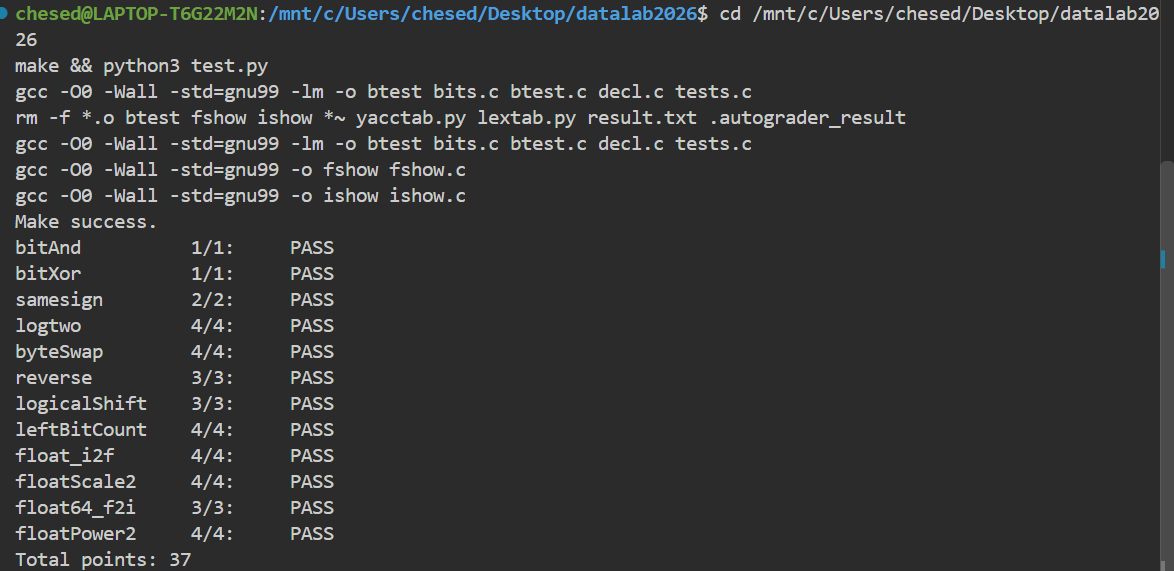
\includegraphics[width=0.94\textwidth]{imgs/test_result.png}
\caption*{test 截图：test.py 全部通过，Total points: 37}
\end{figure}

\section{解题报告}

\subsection{亮点}

下面几道题写的比较久，写一下。有部分内容用了AI。bitXor 是上限卡得最死的一道；logtwo 是合法符号少得反常，常规写法根本用不出来；float\_i2f 的舍入我调了比较久；float64\_f2i 上限给了 60，我只用了 16，是收得比较干净的一道。

\subsection{bitXor}

合法符号只有 \oTilde{} 和 \oAmp，上限 7 个。

我第一遍是把 $x \oplus y$ 拆成两个半边：

\begin{codeblock}
x \cCir{} y = \cTilde(\cTilde(x \cAmp \cTilde{}y) \cAmp \cTilde(\cTilde{}x \cAmp y))
\end{codeblock}

逻辑没问题，btest 也过了，但数了一遍 op 是 8 个，超了一个。后来换了个角度，从集合上看：\code{x \& y} 是交集，\code{x | y} 是并集，而“两位不一样”其实就是并集里挖掉交集，也就是

\begin{codeblock}
x \cCir{} y = (x \cPipe{} y) \cAmp \cTilde(x \cAmp y)
\end{codeblock}

再把 \code{|} 用德摩根换成 \oTilde{} 和 \oAmp，正好 7 个。

两者差的这一个 op 在哪，我想了一下：对称写法里两个半边各要多取一次反，而这一版 \code{\cTilde(x \& y)} 的反是本来就要算的，省的就是它。所以题目上限写 7 应该就是卡在这两条路的差额上，多做一次取反就不够用了。

\subsection{logtwo}

合法符号是 \code{>} \code{<} \code{>>} \code{<<} \code{|}。没有 \oAmp，没有 \code{!}，没有 \code{+}，也没有 \code{if}。

只能换问法。反正比较是允许的，那就别问“第几位是 1”，改成问“这个数还大于某个阈值吗”。比如先看 v 有没有大于 0xFFFF，大于的话答案至少是 16，把 v 右移 16 再往下问；不满足就留着看更小的位。依次试 16、8、4、2、1 五个步长就能覆盖 32 位。

中间改过一次。最早写的是 \code{int t = v \& 0xFFFF;}，想先把低半段取出来再判断，写完才想起来 \oAmp 不在合法符号表里。用ai改成直接拿阈值常量比较之后，反而从 23 个降到 18 个，因为中间的变量和移位都省掉了。

\subsection{float\_i2f}

把整数按位转成单精度浮点。这题麻烦的不是取位，是舍入。

流程是：先特判 0，然后拆出符号、对绝对值循环左移，把最高位的 1 顶到 bit31，移了多少次就记下来当指数用。剩下从高往低取 23 位当尾数，再往下的 8 位是要丢掉的部分。

舍入用 round-to-even，丢掉的那 8 位记作 rnd：

\begin{itemize}
  \item rnd 大于 0x80，超过一半，直接进位；
  \item rnd 等于 0x80 时刚好是一半，看尾数最后一位，是奇数才进位，这样舍入完结果一定是偶数；
  \item 小于 0x80 就正常舍掉。
\end{itemize}

还有个很容易漏的地方：尾数加 1 之后有可能变成 0x800000，这就越过隐含位了，得把尾数清回 0、指数减 1。这一步不写的话绝大多数输入还是对的，只有少数几个会错，随手测不太容易撞上。

测的时候我挑了 0x01000001 和 0x01000003，这两个正好卡在中间，一个该舍一个该进。另外 INT\_MIN 也要注意，取绝对值那一步容易出问题。

\section{反馈/收获/感悟/总结}

全部写完花了大约2个小时。logtwo 和float\_i2f 思考的比较久，最后用了ai给解题思路我自己补充代码，其他难度都还好。

\section{参考的重要资料}

使用deepseek v4.1 Flash修改报告和提供部分解题思路

\end{document}
